\section{Input/Output Module}
\label{chap:io}

Reading and writing meshes from/to files is a feature required by most programmers using a geometry processing library.
As such, \code{lox} offers various functionality for \enquote{IO} (input/output), including file operations.
Most of it is defined in the module \code{lox::io}.

Before implementing the functionality, the following goals were set:

\begin{itemize}
  \item \textbf{Speed}: loading and writing meshes should not waste time or resources needlessly.
  \item \textbf{Convenience}: most of the time, programmers do not care about the specifics of IO and should thus be able to use most of the IO functionality very easily.
  \item \textbf{Flexibility}: somewhat contrasting the previous goal, the IO module should be flexible enough so that it can be used in virtually all situations.
  In particular, users should be able to tweak details of IO operations.
  And even if users need to load unusual data, they should never be required to write their own parser for a specific file format, but instead be able to use the functionality of \code{lox}.
  \item \textbf{More than files}: the IO functionality should not be restricted to files.
  For example, there are sources of mesh data other than files.
  Everything that can provide or receive mesh data should be able to use the IO interface like a file.
  \item \textbf{Correct and robust}: invalid input should never crash the library.
  Instead, an error indicating the problem should be emitted.
  Additionally, reader and writers of file formats should stick to the specification as closely as possible.
  \item \textbf{Compile time correctness}: unless this conflicts with the other goals, as many programmer errors as possible should be caught at compile time.
\end{itemize}

\vfill
A set of traits is required at the core of the IO module in order to abstract over all types that can provide or receive mesh data (including files).
In \code{lox}'s design, everything that can provide mesh data is called a \emph{source}, everything that can receive it is called a \emph{sink}.
The exact design of these traits is of uppermost importance for meeting the goals defined above.

An early important realization is that there are two kinds of sources and sinks each: those which can provide/receive data in any order and those who are restricted to a particular order of data.
For example, files are restricted to the specific order defined by their file format which can differ between different formats, e.\,g., \textsc{Ply} and \textsc{Obj}.
Those files have to be read/written from front to back and usually do not allow random access.
Similarly, meshes defined algorithmically provide the mesh data in the order that the algorithm creates it.
On the other hand, in-memory mesh data structures and property maps allow arbitrary access to their data.

This important distinction is reflected in the trait system by exposing \code{MemSource} and \code{MemSink} (allowing random access) as well as \code{StreamSource} and \code{StreamSink} (restricted to one order).
These traits are also shown in figure~\ref{fig:io-traits}.
This system has some similarities to the \code{Reader}/\code{Writer} and \code{Importer}/\code{Exporter} system of OpenMesh.

\begin{figure}[t]
  \centering
  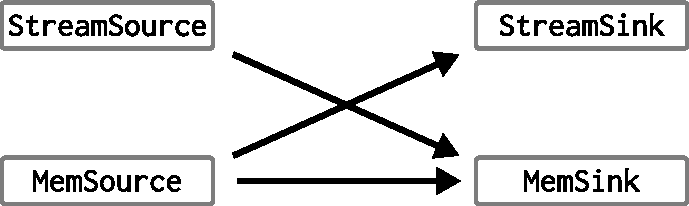
\includegraphics[width=.6\textwidth]{svg2pdf/io-traits}
  \caption{
    The core IO traits of \codebox{lox}.
    To transfer mesh data, the source, the sink or both have to provide random access to the
    data.
  }
  \label{fig:io-traits}
\end{figure}

\newpage

Since the \code{Stream*} versions of these traits are the restricted ones, they have to define the main procedure as this specifies the order of mesh data.
This results in fairly minimal trait interfaces for those two traits:

\begin{rustcode}
  trait StreamSource {
      fn transfer_to<SinkT: MemSink>(self, sink: &mut SinkT) -> Result<(), Error>;
  }

  trait StreamSink {
      fn transfer_from<SrcT: MemSource>(self, src: &SrcT) -> Result<(), Error>;
  }
\end{rustcode}

The \code{Mem*} variants of those traits have a significantly larger interface.
\code{MemSource} contains a method to return a reference to the \enquote{core mesh} (containing the connectivity) which is required to at least implement the traits \code{Mesh} and \code{BasicAdj}.
The trait also contains methods for every predefined mesh property, a list that currently includes vertex positions, vertex normals, vertex colors, face normals and face colors.
The \code{MemSink} has a similar interface that allows adding connectivity and property data.

A difficult part of the design was to allow for different types of mesh properties.
This is required because different file formats store mesh properties with different types and some file formats even allow storing multiple types (e.\,g., \textsc{Ply}).
For example, \code{lox} should be able to read and write \code{f32} \emph{and} \code{f64} vertex positions;
reading and writing color data should work with \code{f32} \emph{and} \code{u8} channels -- with or without alpha channel.
This flexibility was achieved by making all property methods of the \code{Mem*} traits generic and providing a separate method to ask for the preferred data type.
This made the interface notably more complex, but this was accepted in order to provide a fast and flexible core interface.
Ideally, most users do not need to interact with these core traits directly anyway, making the complexity increase less of an issue.

As the core data structures (e.\,g., \code{HalfEdgeMesh}) cannot store mesh properties, external property maps are needed for those.
The user is then supposed to create a struct type that contains the core mesh and all required property meshes.
These types are called \enquote{fat meshes} in the context of \code{lox}.
In order to read mesh data from a file into a fat mesh or to write a fat mesh to a file, the fat mesh type needs to implement \code{MemSource} and \code{MemSink}.
However, implementing those traits is not trivial and requires a lot of boilerplate code.
Requiring the user to write those implementations would make using the library a lot less convenient.

Two features are offered to solve this problem.
First, \code{lox} implements and exposes a few predefined fat meshes in the module \code{lox::fat}.
For example, \code{fat::MiniMesh} stores the core mesh and \code{f32} vertex positions, making it applicable in many situations.
But more importantly, \code{lox} provides a \emph{custom derive} for both \code{Mem*} traits which allows to implement the traits by simply annotating the struct definition.
Example:

\begin{rustcode}
#[derive(MemSource, MemSink)]
struct MyMesh {
    #[lox(core_mesh)]
    mesh: HalfEdgeMesh,

    #[lox(vertex_position)]
    positions: VecMap<VertexHandle, Point3<f32>>,
}
\end{rustcode}

These \emph{custom derives} are implemented as \emph{procedural macros}: functions that operate on the source code and emit new source code.
Unfortunately, completely explaining procedural macros in this chapter is not possible.
In short, a function defined by \code{lox} receives the definition of the struct \code{MyMesh} in form of a token stream, parses it into an abstract syntax tree, inspects it and generates new Rust code in form of a token stream containing an \code|impl Mem* for MyMesh { ... }| block.
This function is called by the compiler during compilation and the generated code is then fed back into the compilation process.
This has the effect, that the \code{Mem*} traits are implemented for \code{MyMesh} without the user having to write any boilerplate code.

Another important part of the IO functionality is \emph{type casting}.
In a fat mesh, the types of mesh properties are usually fixed, e.\,g., \code{Point3<f32>} vertex positions or \code{[u8; 3]} colors.
As files may contain or require properties with a different type, the IO code should be able to deal with that type mismatch.
One possibility is to always convert between the types automatically.
While this makes the interface more convenient to use (as the problem is not exposed), it could exhibit behavior unexpected by the user.
Casting between different numeric types often requires clamping or rounding (cf. figure~\ref{fig:casting}), something the user might want to prevent or at least know about.

As with the order of data, the type of properties is ultimately determined by the \code{Stream*} sinks and sources, meaning that the responsibility for type casting lies with the \code{Mem*} part.
Those can either cast to the destination type or raise an error if they cannot handle that specific type conversion.
To make this choice easily available to the user, the custom derives support annotating one of five \emph{casting modes}: \code{none}, \code{lossless}, \code{clamping}, \code{rounding} and \code{lossy} -- the last one is the default and allows casts involving both, clamping and rounding.
A simple example:

\begin{rustcode}
#[lox(vertex_normal, cast = "lossless")]
vertex_normals: VecMap<VertexHandle, Vector3<f32>>,
\end{rustcode}

\newpage

\begin{figure}[t]
  \centering
  \setlength{\dashlinedash}{.3mm}
  \setlength{\dashlinegap}{.6mm}
  \setlength{\tabcolsep}{0mm}

  \newcommand{\lossless}{\raisebox{-.5mm}{\tikz[scale=0.15]{\fill[flat-green-light] (0,0) circle(1);}}}
  \newcommand{\clamping}{\raisebox{-.5mm}{\tikz[scale=0.15]{\fill[flat-red-light] (0,0) circle(1);}}}
  \newcommand{\rounding}{\raisebox{-.5mm}{\tikz[scale=0.15]{\fill[flat-gray-dark] (0,0) circle(1);}}}
  \newcommand{\lossy}{%
    \raisebox{-1mm}{%
      \tikz[rotate=45, scale=0.15]{%
        \begin{scope}%
          \clip (-1,0) rectangle (1,1);%
          \fill[flat-red-light] (0,0) circle(1);%
        \end{scope}%
        \begin{scope}%
          \clip (-1,0) rectangle (1,-1);%
          \fill[flat-gray-dark] (0,0) circle(1);%
        \end{scope}%
      }%
    }
  }

  \renewcommand{\arraystretch}{0.91}
  \begin{tabular}{|c|C{9mm}:C{9mm}:C{9mm}:C{9mm}:C{9mm}|C{9mm}:C{9mm}:C{9mm}:C{9mm}:C{9mm}|C{9mm}:C{9mm}|}\hline
    \hfill \textbf{$\lcurvearrowne$} \hspace{0mm}
      & \textbf{\codebox{u8}} & \textbf{\codebox{u16}} & \textbf{\codebox{u32}}
      & \textbf{\codebox{u64}} & \textbf{\codebox{u128}}
      & \textbf{\codebox{i8}} & \textbf{\codebox{i16}} & \textbf{\codebox{i32}}
      & \textbf{\codebox{i64}} & \textbf{\codebox{i128}}
      & \textbf{\codebox{f32}} & \textbf{\codebox{f64}}\\\hline

      \textbf{\codebox{u8}}
        & \lossless & \lossless & \lossless & \lossless & \lossless
        & \clamping & \lossless & \lossless & \lossless & \lossless
        & \lossless & \lossless \\\hdashline
      \textbf{\codebox{u16}}
        & \clamping & \lossless & \lossless & \lossless & \lossless
        & \clamping & \clamping & \lossless & \lossless & \lossless
        & \lossless & \lossless \\\hdashline
      \textbf{\codebox{u32}}
        & \clamping & \clamping & \lossless & \lossless & \lossless
        & \clamping & \clamping & \clamping & \lossless & \lossless
        & \rounding & \lossless \\\hdashline
      \textbf{\codebox{u64}}
        & \clamping & \clamping & \clamping & \lossless & \lossless
        & \clamping & \clamping & \clamping & \clamping & \lossless
        & \rounding & \rounding \\\hdashline
      \textbf{\codebox{u128}}
        & \clamping & \clamping & \clamping & \clamping & \lossless
        & \clamping & \clamping & \clamping & \clamping & \clamping
        & \rounding & \rounding \\\hline
      \textbf{\codebox{i8}}
        & \clamping & \clamping & \clamping & \clamping & \clamping
        & \lossless & \lossless & \lossless & \lossless & \lossless
        & \lossless & \lossless \\\hdashline
      \textbf{\codebox{i16}}
        & \clamping & \clamping & \clamping & \clamping & \clamping
        & \clamping & \lossless & \lossless & \lossless & \lossless
        & \lossless & \lossless \\\hdashline
      \textbf{\codebox{i32}}
        & \clamping & \clamping & \clamping & \clamping & \clamping
        & \clamping & \clamping & \lossless & \lossless & \lossless
        & \rounding & \lossless \\\hdashline
      \textbf{\codebox{i64}}
        & \clamping & \clamping & \clamping & \clamping & \clamping
        & \clamping & \clamping & \clamping & \lossless & \lossless
        & \rounding & \rounding \\\hdashline
      \textbf{\codebox{i128}}
        & \clamping & \clamping & \clamping & \clamping & \clamping
        & \clamping & \clamping & \clamping & \clamping & \lossless
        & \rounding & \rounding \\\hline
      \textbf{\codebox{f32}}
        & \lossy & \lossy & \lossy & \lossy & \lossy
        & \lossy & \lossy & \lossy & \lossy & \rounding
        & \lossless & \lossless \\\hdashline
      \textbf{\codebox{f64}}
        & \lossy & \lossy & \lossy & \lossy & \lossy
        & \lossy & \lossy & \lossy & \lossy & \lossy
        & \lossy & \lossless \\\hline
  \end{tabular}
  \renewcommand{\arraystretch}{1.0}
  \caption{
    Casts between numerical types.
    For some conversion, some values might need to be clamped\,\protect\clamping{}, rounded\,\protect\rounding{} or both\,\protect\lossy to be representable in the target type.
    If all values of the source type can exactly be represented in the target type, it is marked with \protect\lossless{}.
  }
  \label{fig:casting}
\end{figure}

For each file format, \code{lox} defines a \code{Reader} and \code{Writer} which implement \code{StreamSource} and \code{StreamSink}, respectively.
The four sink/source traits constitute the mid-level IO interface: it is already abstracted, but still not particularly easy to use.
As low-level interface, each \code{Reader} and \code{Writer} exposes format-specific methods which allow reading data of that format without the source/sink interface.
To provide a convenient high-level interface, too, a couple of functions are directly exported by the IO module, including the following ones (here slightly simplified):

\begin{rustcode}
fn read_file<SinkT: Empty + MemSink>(path: &Path)
    -> Result<SinkT, Error>
{ … }

fn write_file<SrcT: MemSource>(path: &Path, src: &SrcT)
    -> Result<(), Error>
{ … }
\end{rustcode}

This allows users to write \code{let mesh: MyMesh = io::load_file("foo.ply");}, for example.
That code automatically detects the correct file format, instantiates the corresponding \code{Reader}, uses the source/sink traits to transfer mesh data and returns the new \code{MyMesh} instance.

\vspace{1.5cm}

Currently, \code{lox} has full support for the \textsc{Ply} and \textsc{Stl} file formats, with more file formats (including \textsc{Obj}) planned for the near future.
To guarantee a high implementation quality and adherence to the (unfortunately often very imprecise) format specifications, different tests are used.
For one, a number of unit tests read and write various meshes with various properties and check if the written file or the loaded mesh is correct.

Furthermore, so called \emph{fuzzing} tests are used.
In those, a \emph{fuzzer} automatically generates a large number of inputs that are given to the parsers of the different file formats.
The inputs are not completely random, however.
Instead, the fuzzer tries to achieve a high code coverage by analyzing which statements and branches are executed for what inputs and then tries to systematically generate inputs to reach previously unreached code.
That way, advanced fuzzers can generate valid input files from just analyzing and trying to optimize code coverage (cf. \cite{jpegfuzzing}).

The goal of fuzzing tests is usually to find crashes and other unexpected behavior.
This is particularly useful for parsers, as they often have to deal with many obscure edges cases.
Due to fuzzing tests, a couple of bugs were found and fixed in \code{lox}'s parsers.



\vspace{1.5cm}


With this core system of traits and the three different layers of convenience/abstraction, all initial goals are met for the most part.
There are still a number of possible improvements, but the system as offered is already fairly fast, flexible and convenient to use.
\vspace{6mm}
